\documentclass[xcolor=dvipsnames,aspectratio=169]{beamer}
\usecolortheme[dark,accent=cyan]{solarized}
\usepackage[utf8]{inputenc}
\usepackage{multicol}
\usepackage{url}
\usepackage{hyperref}
\usepackage{subfig}
\title{Cryptography}
\author{Gaspare Ferraro\\ ferraro@gaspa.re}
\subtitle{Hackers ahead of time}

\begin{document}

\begin{frame}[plain]
\maketitle
\begin{columns}
\column{0.5\textwidth}
	\center {
		\includegraphics[width=0.3\textwidth]{style/qrcode.png}\\
		Visit us!
		}
\column{0.5\textwidth}
	\center{
		\includegraphics[width=0.3\textwidth]{style/gaspare.jpg}\\
		@GaspareG
	}
	
\end{columns}
\end{frame}

%%%%%%%%%%%%%%%%%%%%%%%%%%%%%%%%%%%%%%%%%%%%%%%%%%%%%%%%%%%%%%%%%%%%%%%%%%%%%%%
%%%%%%%%%%%%%%%%%%%%%%%%%%%%%%%%%%%%%%%%%%%%%%%%%%%%%%%%%%%%%%%%%%%%%%%%%%%%%%%

\part{Introduzione}

\begin{frame}
	\partpage
	\centering
\end{frame}

\begin{frame}{Warning!}

  \center {
    In questo incontro si fa uso della {\color{red} \textit{matematica}}! 
    
    \medskip
    
    \pause

    \includegraphics[width=0.5\textwidth]{img/meme}
    
    \medskip
    
    \pause

    Non è sempre stato così però...
  }
  
\end{frame}

\begin{frame}{La crittografia ieri}
    
  \pause

  \begin{figure}%
    \centering
    \subfloat[Cifrario di Cesare]{{
  \centering\includegraphics[width=5cm]{img/cesaer.png} }}%
  \pause
    \qquad
    \subfloat[Scitala]{{
  \centering\includegraphics[width=5cm]{img/scitala.png} }}%
    %\caption{2 Figures side by side}%
    %\label{fig:example}%
  \end{figure}


\end{frame}

\begin{frame}{La crittografia oggi}
  \center {
    Le necessità, così come le risorse a disposizione, si sono evolute 
    
    ed oggi possiamo suddividere la crittografia in:
     
    \pause
    
    \medskip
    \includegraphics[width=0.6\textwidth]{crypto-section.pdf}
  }
\end{frame}
%%%%%%%%%%%%%%%%%%%%%%%%%%%%%%%%%%%%%%%%%%%%%%%%%%%%%%%%%%%%%%%%%%%%%%%%%%%%%%%
%%%%%%%%%%%%%%%%%%%%%%%%%%%%%%%%%%%%%%%%%%%%%%%%%%%%%%%%%%%%%%%%%%%%%%%%%%%%%%%

\part{Crittografia simmetrica}

\begin{frame}
	\partpage
	\centering
\end{frame}

\begin{frame}{Crittografia simmetrica}

  I cifrari simmetrici sono quelli dove i messaggi $m$ vengono cifrati e decifrati usando una stessa chiave $k$, che deve essere nota esclusivamente alle due parti.
  
  \medskip

  $\mathcal{C}(m, k) = c$ (funzione di cifratura)
    
  $\mathcal{D}(c, k) = m$ (funzione di decifratura)
  
  \medskip

  Ovviamente deve valere che:
  
  $\mathcal{D}(\mathcal{C}(m, k), k) = m$ (il messaggio originale non viene alterato durante lo scambio).
  
  \medskip
  
  Per esempio nel cifrario di Cesare:
  
  $\mathcal{C}(m, k) = $ ruota in avanti di $k$ ogni singolo carattere.
  
  $\mathcal{D}(c, k) = $ ruota indietro di $k$ ogni singolo carattere.
  
\end{frame}

\begin{frame}{XOR cipher}

\end{frame}

\begin{frame}{Crittoanalisi statistica}
  Spesso le vulnerabilità non è nell'algoritmo ma nella sua applicazione...
  
  \begin{itemize}
    \item 
  \end{itemize}
\end{frame}

\begin{frame}{One-time Pad}
  
  Il Cifrario di Vernam .
  
  Chiamato anche one-time pad poichè
  
\end{frame}

%%%%%%%%%%%%%%%%%%%%%%%%%%%%%%%%%%%%%%%%%%%%%%%%%%%%%%%%%%%%%%%%%%%%%%%%%%%%%%%
%%%%%%%%%%%%%%%%%%%%%%%%%%%%%%%%%%%%%%%%%%%%%%%%%%%%%%%%%%%%%%%%%%%%%%%%%%%%%%%

\part{Crittografia asimmetrica}

\begin{frame}
	\partpage
	\centering
\end{frame}

\begin{frame}{Concetti base}
  La crittografia asimmetrica si basa sulle funzioni \textit{one-way trapdoor} e sulla presenza di una coppia di chiavi (chiamate chiave pubblica e chiave privata).
  
  \pause
  
  \medskip
  
  Una funzione $f$ si dice \textit{trapdoor} se: 
  \begin{itemize}
    \item Calcolare $y = f(x)$ è computazionalmente facile.
    \item Calcolare $x = f^{-1}(y)$ è computazionalmente difficile \textit{(senza nessuna informazione aggiuntiva)}.
  \end{itemize}

  \pause
  
  \smallskip
  
  Un esempio è il problema della fattorizzazione:
  \begin{itemize}
    \item $m = f(\{p, q\}) = (p \times q)$ (calcolo del prodotto tra i primi $p$ e $q$).
    \item $\{p, q\} = f^{-1}(n) =\ {\color{red}??} $ (scomposizione in fattori primi di $n$).
  \end{itemize}
    
  \smallskip
  
  \pause
  
  $f(\{49171, 61843\}) = 3040882153$ (facile quanto aprire una calcolatrice).
  $f^{-1}(1841488427) = ??$ (devo provare tutti i divisori da $2$ a $\sqrt{n}$).
  
  \pause
  
  Il problema diventa banale se conosco uno dei due divisori:
  $1841488427 / 58049 = 31723$

\end{frame}

\begin{frame}{Aritmetica modulare}

Diciamo che due interi $a$ e $b$ sono congrui modulo $n$, scritto $a \equiv b$ (mod $n$), se

$(a\ \%\ n) = (b\ \%\ n)$ dove \% è il resto della divisione intero (modulo).

\medskip

\pause

Alcune proprietà matematiche:

\pause

\begin{itemize}
  \item $a + k\equiv b + k$ (mod $n$), invariante per addizione.
  \item $k*a \equiv k*b$ (mod $n$), invariante per moltiplicazione.
  \item $a^k \equiv b^k$ (mod $n$), invariante per potenza.\pause
  \item $\sqrt{a} \equiv b$ (mod $n$) se $a \equiv b^2$ (mod $n$), radice quadrata.
  \item $a^{-1} \equiv b$ (mod $n$) se $ab \equiv 1$ (mod $n$), inverso moltiplicativo.
  \item ...
\end{itemize}

\end{frame}

\begin{frame}{RSA pt.1}

\pause

L'algoritmo di cifratura asimmetrica più famoso è l'RSA (da {\color{red}R}ivest {\color{red}S}hamir {\color{red}A}dleman) che si basa sul problema della fattorizzazione e sull'algebra modulare.

\pause

\smallskip

Il funzionamento di base è:\pause

\begin{itemize}
  \item Si scelgono due numeri primi a caso $p$ e $q$ (in modo \textit{sicuro}).\pause
  \item Si calcola il prodotto $n = p*q$ (che sarà il nostro modulo).\pause
  \item Si calcola il toziente $\phi(n) = (p-1)*(q-1)$ (il numero dei coprimi con $n$).\pause
  \item Si sceglie a caso un numero $e$, coprimo e minore di $\phi(n)$.\pause
  \item Si calcola il numero $d$ come inverso moltiplicativo di $e$, ovvero $ed \equiv 1$ (mod $\phi(n)$).
\end{itemize}

\medskip

\pause

Chiamiamo quindi:

\pause

$k_{pub} = (n, e)$ la chiave pubblica che distribuiamo.

\pause

$k_{priv} = (n, d)$ la chiave privata che teniamo segreta.

\end{frame}

\begin{frame}{RSA pt.2}

Una volta calcolata la chiave pubblica e quella privata possiamo cifrare e decifrare i messaggi in questo modo:

\pause
\medskip

$\mathcal{C}(m, k_{pub}) = m^{e} $ (mod $n$) \pause
  
$\mathcal{D}(c, k_{priv}) = c^{d} $ (mod $n$)

\medskip

\pause

Si ma perchè funziona?

\medskip

\pause

Dal teorema di Eulero sappiamo che $m^{\phi(n)} \equiv 1 $ (mod $n$).

I valori $e$ e $d$ sono calcolati in modo che $ed \equiv 1$ (mod $\phi(n)$).

\medskip

$\mathcal{D}(\mathcal{C}(m, k), k) = m^{ed} = m^{\phi(n)*t + 1} = m^{\phi(n)^{t}} * m = 1 * m = m$

\end{frame}

\begin{frame}{Un esempio per capire}
  
\pause

  Scegliamo i sequenti parametri:
  
  \begin{itemize}
    \item $p = 13$ e $q = 23$
    \item $n = p*q = 299$
    \item $\phi(n) = (13-1)*(23-1) = 264$
    \item $e = 7$, $\gcd(264, 7) = 1$
    \item $d = 151$, $7*151 \equiv 1 $ (mod $264$)
  \end{itemize}
  
  \smallskip
  
\pause

  Quindi $k_{pub} = (299, 7)$ e $k_{priv} = (299, 151)$. Vogliamo cifrare $m = 42$.
  
\pause

  \medskip
  
  $\mathcal{C}(m, k_{pub}) = m^{e} = 42^7 = 230539333248 = 107$ (mod $299$) 
 
 \pause
  
  $\mathcal{D}(c, k_{priv}) = c^{d} = 107^{151} = 2743956545...948643 = 42 $ (mod $299$)

\end{frame}

\begin{frame}{(Non tanto) a caso}

\pause

"Si scelgono due numeri primi \textit{a caso} $p$ e $q$ (in modo \textit{sicuro})"

\begin{itemize}
  \item Scegliere $p$ e $q$ di almeno $1024$ bit.
  \item Scegliere $p$ e $q$ non troppo vicini tra loro.
  \item Non riusare uno dei primi per altri moduli.
\end{itemize}

\smallskip
\pause
Con la potenza di calcolo attuale è possibile fattorizzare semiprimi fino a (circa) $768$ bit, i moduli più grandi sono (per ora) resistenti agli attacchi bruteforce.

\smallskip
\pause
Se $p$ e $q$ sono vicini allora abbiamo che $n \simeq p^2 \simeq q^2$ e quindi anche $\sqrt{n}$ sarà vicino ai primi. Basterà quindi un attacco bruteforce che cerca i fattori vicino alla radice quadrata.

\smallskip
\pause

Se $n_1 = p*q^{'}$ e $n_2 = p*q^{''}$ allora $p = \gcd(n_1, n_2)$.

\end{frame}

%%%%%%%%%%%%%%%%%%%%%%%%%%%%%%%%%%%%%%%%%%%%%%%%%%%%%%%%%%%%%%%%%%%%%%%%%%%%%%%
%%%%%%%%%%%%%%%%%%%%%%%%%%%%%%%%%%%%%%%%%%%%%%%%%%%%%%%%%%%%%%%%%%%%%%%%%%%%%%%

\part{Hashing}

\begin{frame}
	\partpage
	\centering
\end{frame}

\begin{frame}{Creare confusione}

Chiamiamo hash una funzione \textit{non invertibile} che associa 

\begin{itemize}
  \item Resis
\end{itemize}


\pause

Funzioni di hash famose sono l'MD5, SHA-1, SHA-256, SHA-384, ...

\pause

Utilizzi pratici:

\begin{itemize}
  \item Salvataggio delle password (preferibilmente con un salt).
  \item Creazione di hashtable (struttura dati con accesso diretto).
  \item Controllo di integrità (\textit{md5sum}, \textit{sha1sum}).
  \item Firma digitale (sull'hash invece che sul documento).
\end{itemize}

\end{frame}

\begin{frame}{Alla ricerca dell'inversa}
  
\end{frame}

\begin{frame}{Un (pessimo) esempio...}
    \pause

  \begin{figure}%
    \centering
    \subfloat{{
  \centering\includegraphics[width=7cm]{img/trenitalia2} }}%
  \pause
    \qquad
    \subfloat{{
  \centering\includegraphics[width=5cm]{img/trenitalia} }}%
    %\caption{2 Figures side by side}%
    %\label{fig:example}%
  \end{figure}

\end{frame}
%%%%%%%%%%%%%%%%%%%%%%%%%%%%%%%%%%%%%%%%%%%%%%%%%%%%%%%%%%%%%%%%%%%%%%%%%%%%%%%
%%%%%%%%%%%%%%%%%%%%%%%%%%%%%%%%%%%%%%%%%%%%%%%%%%%%%%%%%%%%%%%%%%%%%%%%%%%%%%%
\begin{frame}{Fine}

\end{frame}
%%%%%%%%%%%%%%%%%%%%%%%%%%%%%%%%%%%%%%%%%%%%%%%%%%%%%%%%%%%%%%%%%%%%%%%%%%%%%%%
%%%%%%%%%%%%%%%%%%%%%%%%%%%%%%%%%%%%%%%%%%%%%%%%%%%%%%%%%%%%%%%%%%%%%%%%%%%%%%%

\end{document}
